\task{Stetigkeit}{4}
Untersuche, in welchen Punkten die Funktion $f:\RR\to\RR$ stetig ist. Fertige auch eine Skizze an.
\[
f(x)=
\begin{cases}
    -x & \text{falls $x<0$ oder $x>1$,} \\
    x^2 & \text{sonst.}
\end{cases}
\]

\begin{solution}
    Da $-x$ und $x^2$ jeweils Polynome sind und Polynome auf ganz $\RR$ stetig sind, müssen wir nur die Grenzfälle $x\to0$ und $x\to1$ anschauen. \\
    Schauen wir uns zuerst $x\to0$ an: 
    \[\lim_{x\to0^-}f(x)=\lim_{x\to0^-}-x=0\]
    \[\lim_{x\to0^+}f(x)=\lim_{x\to0^+}x^2=0^2=0\]
    $\Rightarrow f(x)$ ist stetig im Punkt $x=0$ \\
    Als nächstes schauen wir uns $x\to1$ an:
    \[\lim_{x\to1^-}f(x)=\lim_{x\to1^-}x^2=1^2=1\]
    \[\lim_{x\to1^+}f(x)=\lim_{x\to1^+}-x=-1\] 
    $\Rightarrow f(x)$ ist nicht stetig im Punkt $x=1$. \\
    Folgende Grafik ist eine Skizze von $f(x)$:
    \begin{center}
        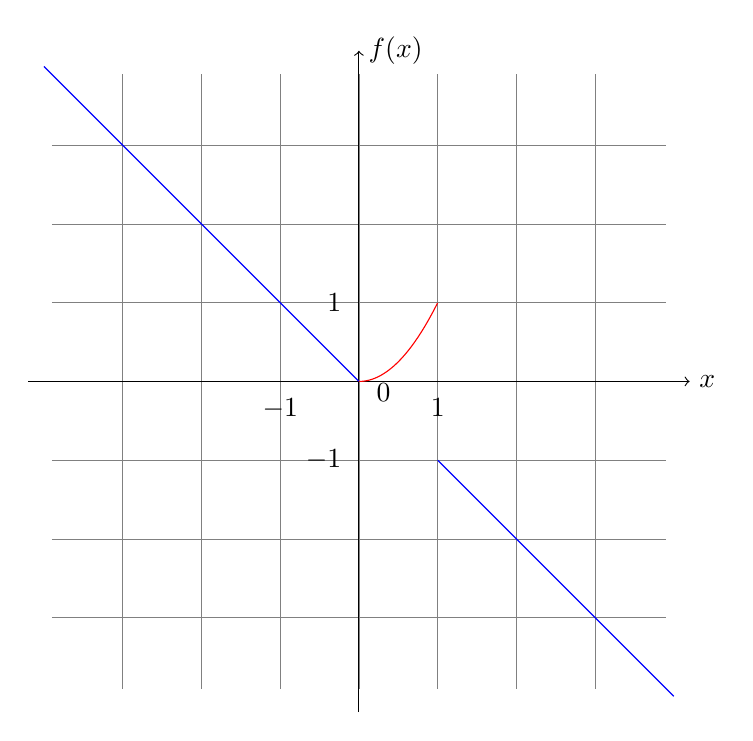
\begin{tikzpicture}[domain=-4:4]
        % Grid(dy)
        \draw[very thin, color=gray] (-3.9,-3.9) grid (3.9,3.9);
        \draw[->] (-4.2,0) -- (4.2,0) node[right] {$x$};
        \draw[->] (0,-4.2) -- (0,4.2) node[right] {$f(x)$};

        % Labels
        \node at (0.1,0.1) [below right] {$0$};
        \node at (1,-0.1) [below] {$1$};
        \node at (-1,-0.1) [below] {$-1$};  
        \node at (-0.1,1)[left] {$1$};
        \node at (-0.1,-1)[left] {$-1$};

        % Graph
        \draw[color=blue, domain = -4:0, samples = 100, smooth] plot (\x,{-\x});  
        \draw[color=blue, domain = 1:4, samples = 100, smooth] plot (\x,{-\x});
        
        \draw[color=red, domain=0:1, samples=100, smooth] plot (\x,{\x^2});
        
        \end{tikzpicture}
    \end{center}
\end{solution}